\subsection{Object-sorting: Robustness and Out-of-Distribution generalization}
In this experiment, we evaluate robustness to a particular type of noisy corruption. We train each model on the same
object-sorting task described above. We use a fixed training set size of $3,000$ for the same reason---it
is large enough that all models are able to learn the task. On the hold out test set, we corrupt the object
representations by applying a random linear transformation. In particular, we randomly sample a random matrix the
entries of which are iid zero-mean Gaussian with variance $\sigma^2$, $\Phi \in \mathbb{R}^{d \times d}, \Phi_{ij} \sim \mathcal{N}(0, \sigma^2)$. Each object in $\mathcal{O}$ is then corrupted by this random linear transformation,
$\tilde{o}_i = \Phi o_i, \ \text{ for each } i \in [48]$. We also test robustness to additive noise via $\tilde{o}_i = o_i + \varepsilon_i, \varepsilon_i \sim \mathcal{N}(0, \sigma^2 I_d)$.

The models are evaluated on the hold-out test set with objects replaced by their corrupted version. We evaluate the sorting accuracy of each model while varying the noise level $\sigma$ (5 trials at each noise level). The results are shown in figures~\ref{fig:exp_robustness1} and~\ref{fig:exp_robustness2}. We emphasize that the models are trained only on the original objects in $\mathcal{O}$, and are not trained on objects corrupted by any kind of noise.

This experiment can be interpreted in two lights: the first is robustness to noise. The second is a form of out-of
-distribution generalization. Note that the objects seen by the models post-corruption lie in a different space than
those seen during training. Hence the models need to learn relations that
are in some sense independent of the value representation.
As a theoretical justification for this behavior,~\cite{zhouCompressedPrivacySensitive2009} shows that $\langle \Phi x, \Phi y \rangle \approx \langle x, y \rangle$ in high dimensions, for a random matrix $\Phi$ with iid Gaussian entries. This indicates that models whose primary computations are performed via inner products, like Abstractors, may be more robust to this kind of corruption.

\begin{figure}[ht]
    \begin{subfigure}[t]{0.40\textwidth}
        %\centering
        \hskip-.35in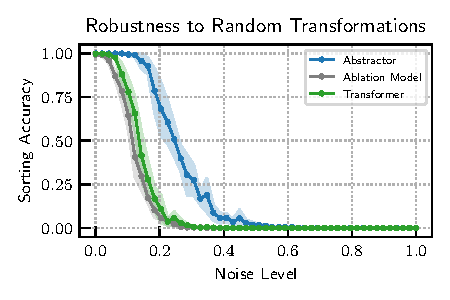
\includegraphics[scale=.95]{figures/experiments/additive_robustness.pdf}
        \vskip-5pt
        \caption{The Abstractor is more robust to corruption by additive noise. }\label{fig:exp_robustness1}
    \end{subfigure}\hspace{\fill}
    \begin{subfigure}[t]{0.40\textwidth}
        %\centering
        \hskip-.6in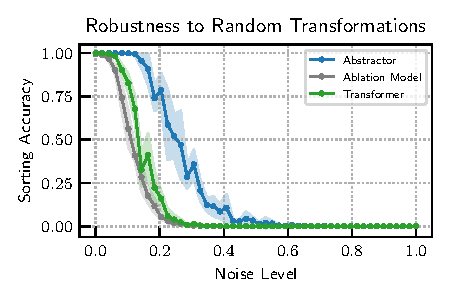
\includegraphics[scale=.95]{figures/experiments/multiplicative_robustness.pdf}
        \vskip-5pt
        \caption{The Abstractor is more robust to corruption by a random linear transformation.}\label{fig:exp_robustness2}
    \end{subfigure}
    \caption{Experiments on robustness and ``out-of-distribution'' generalization.}\label{fig:exp_robustness}
\end{figure}